\chapter{Implementation and Assessment}
\label{chp:Implementation_and_Assessment}

All algorithms discussed in this work are realized in \mbox{MATLAB}, a programming language specialized on matrix manipulations.
It is especially useful for high-dimensional matrix operations, such as the ones for this work.
The following text explains the implementation of the theoretical models and concepts discussed in the previous chapters.
For the implementation, the goal was to make the pipeline as flexible as possible to support all kinds of light fields in different formats.

\section{Requirements}
\label{sec:requirements}

For the implementation and physical realization, some assumptions and requirements have to be formulated.
The input light field for the optimization algorithm is expected to be a five dimensional array $L$ with entries $L_{ijklc}$, where pairs $(i, j)$ and $(k, l)$ correspond to the angular- and spatial coordinates, and $c$ indexes the color channel. 
The data is normalized such that $L_{ijklc} \in \left[0, 1\right]$.
It is also assumed that the light field is rectified such that indices $i, j$ conform to global coordinates on the $(s, t)$-plane as explained in section~\ref{sec:light_field_aquisition}.
In addition, the baseline as well as the distance between the two planes are a required input for the system.

The attenuator is defined by the number of layers, resolution, size and thickness.
Each layer has the same dimensions and resolution and is modeled to be infinitely thin.
Also, the backlight is modeled as a constant white light field, $L_0 \equiv 1$.

\section{The Basic Procedure}
\label{sec:basic_procedure}

As described in section~\ref{sec:ray_casting}, the two virtual planes that parameterize the light field are placed relative to the attenuator and by ray casting, the entries of the propagation matrix $P$ are computed.
Next, the constrained optimization problem given in equation~\ref{eq:minimize_norm} is solved independently for each color channel using an iterative solver of choice, e.g. \mbox{SART}.
The outcome of each optimization is a vector $\alpha_c$ containing the attenuation values in the interval $\left[ 0, \infty \right)$ where $c = 1, 2, 3$ (red, green, blue) denotes the color channel.
The transmittance values are then obtained by element-wise exponentiation, $t = \exp(-\alpha)$, which holds values between zero and one.
Finally, the linearly indexed vector $t$ is reshaped so that the layers can be extracted as three-dimensional matrices and printed on transparencies.

In order to evaluate the attenuation masks, one has to compare the emitted light field $L^\ast = \exp(- P \alpha)$ with the original, $L$.
For instance, one could evaluate the squared 2-norm of the difference $L - L^\ast$ in each color channel.
However, this resulting number is not very meaningful because it also varies with the size of the light field, i.e. the angular and spatial resolution.
This makes it harder to compare the display quality between different light fields.
Thus, it is better to use a normalized figure such as the mean squared error \mbox{(MSE)} or the root-mean-square error \mbox{(RMSE)} defined as
\begin{equation*}
	\text{MSE} \coloneqq \frac{1}{n} \sum_{i = 1}^{n} (X - X^\ast)^2 = \frac{1}{n} \lVert X - X^\ast \rVert^2
	\quad \text{and} \quad
	\text{RMSE} \coloneqq \sqrt{\text{MSE}}
\end{equation*}
for vectors $X, X^\ast \in \mathbb{R}^n$.
To deal with the color channels, the \mbox{MSE} is computed for each color component and then averaged.

\section{Oversampling}
\label{sec:oversampling}

\section{Baseline Scaling and Back Projection}
\label{sec:baseline_scaling}

Often it is the case that the light field of interest has a depth range that does not match the depth of field of the display because of its fixed thickness.
As a consequence, objects outside the depth of field appear blurry.
This effect is demonstrated in figure~\ref{fig:baseline_scaling} for two different baseline scales.
\begin{figure}[tb]
	\begin{subfigure}{0.5\textwidth}
		\centering
		\documentclass{standalone}
\usepackage{tikz}
\usetikzlibrary{intersections}

\begin{document}
	\begin{tikzpicture}[line width = 0.3mm]
	
	\node[anchor = center, inner sep = 0, outer sep = 0] (I) at (0, 0) {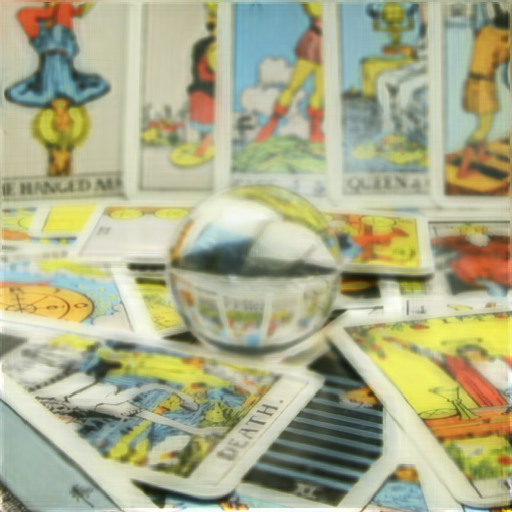
\includegraphics[width = 3.75cm]{../Figures/depth_compression/baseline_unscaled/Reconstruction_of_view_(9,9).png}};
	
	\coordinate (A1) at (-0.6, -1.7);
	\coordinate (S1) at (1, 1);
	\coordinate (A2) at (-1.7, 0.2);
	\coordinate (S2) at (1, 1);
	
	\draw[red]  (A1) rectangle ++(S1); 	
	\draw[blue] (A2) rectangle ++(S2); 
	
	% Magnification box 1
	\node[anchor = south west, xshift = 0.1cm, inner sep = 0pt, outer sep = 0pt, scale = 1.825] (box1) at (I.south east) {
		
		\begin{tikzpicture}
			\begin{scope}
				\clip(A1) rectangle ++(S1);
				\node[anchor = center, inner sep = 0pt] (I) at (0, 0) {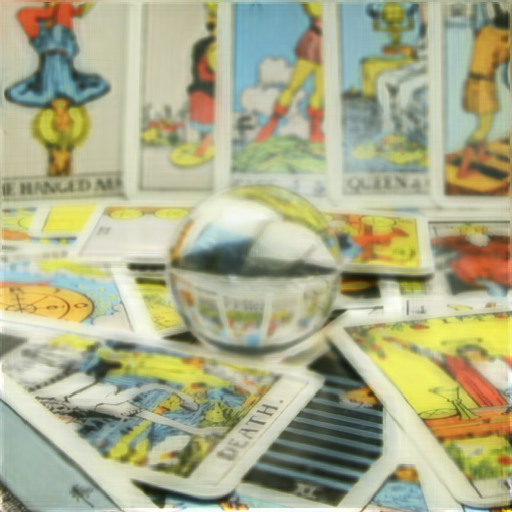
\includegraphics[width = 3.75cm]{../Figures/depth_compression/baseline_unscaled/Reconstruction_of_view_(9,9).png}};
			\end{scope}	
		\end{tikzpicture}
	};
	\draw[red] (box1.south east) rectangle (box1.north west);
	
	% Magnification box 2
	\node[anchor = north west, xshift = 0.1cm, inner sep = 0pt, outer sep = 0pt, scale = 1.825] (box2) at (I.north east) {
		
		\begin{tikzpicture}
			\begin{scope}
				\clip(A2) rectangle ++(S2);
				\node[anchor = center, inner sep = 0pt] (I) at (0, 0) {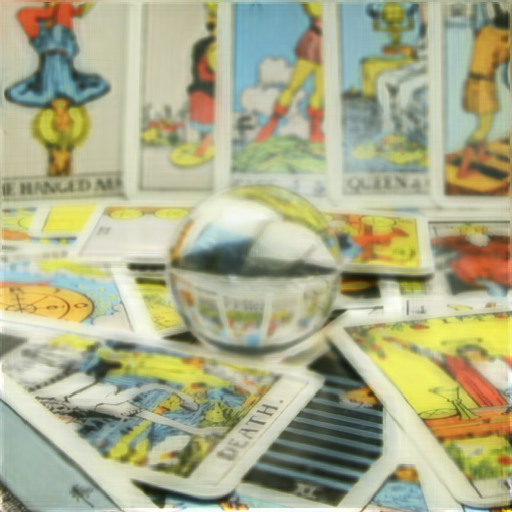
\includegraphics[width = 3.75cm]{../Figures/depth_compression/baseline_unscaled/Reconstruction_of_view_(9,9).png}};
			\end{scope}	
		\end{tikzpicture}
	};
	\draw[blue] (box2.south east) rectangle (box2.north west);
			
	
	\end{tikzpicture}
\end{document}

		\caption{}
		\label{fig:reconstruction_baseline_unscaled}
	\end{subfigure}%
	\begin{subfigure}{0.5\textwidth}
		\centering
		\documentclass{standalone}
\usepackage{tikz}
\usetikzlibrary{intersections}

\begin{document}
	\begin{tikzpicture}[line width = 0.3mm]
	
	\node[anchor = center, inner sep = 0, outer sep = 0] (I) at (0, 0) {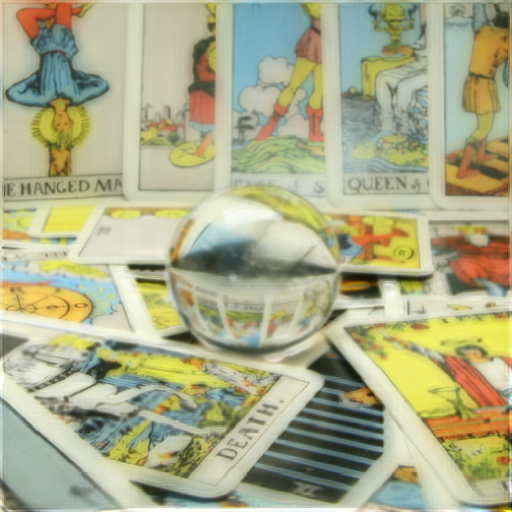
\includegraphics[width = 3.75cm]{../Figures/depth_compression/baseline_scaled_shifted/Reconstruction_of_view_(9,9).png}};
	
	\coordinate (A1) at (-0.6, -1.7);
	\coordinate (S1) at (1, 1);
	\coordinate (A2) at (-1.7, 0.2);
	\coordinate (S2) at (1, 1);
	
	\draw[red]  (A1) rectangle ++(S1); 	
	\draw[blue] (A2) rectangle ++(S2); 
	
	% Magnification box 1
	\node[anchor = south west, xshift = 0.1cm, inner sep = 0pt, outer sep = 0pt, scale = 1.825] (box1) at (I.south east) {
		
		\begin{tikzpicture}
			\begin{scope}
				\clip(A1) rectangle ++(S1);
				\node[anchor = center, inner sep = 0pt] (I) at (0, 0) {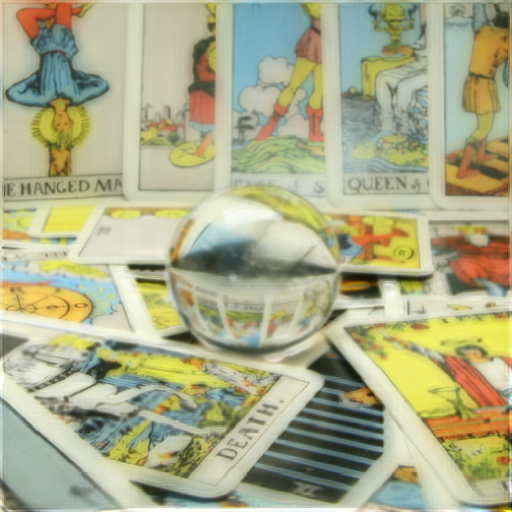
\includegraphics[width = 3.75cm]{../Figures/depth_compression/baseline_scaled_shifted/Reconstruction_of_view_(9,9).png}};
			\end{scope}	
		\end{tikzpicture}
	};
	\draw[red] (box1.south east) rectangle (box1.north west);
	
	% Magnification box 2
	\node[anchor = north west, xshift = 0.1cm, inner sep = 0pt, outer sep = 0pt, scale = 1.825] (box2) at (I.north east) {
		
		\begin{tikzpicture}
			\begin{scope}
				\clip(A2) rectangle ++(S2);
				\node[anchor = center, inner sep = 0pt] (I) at (0, 0) {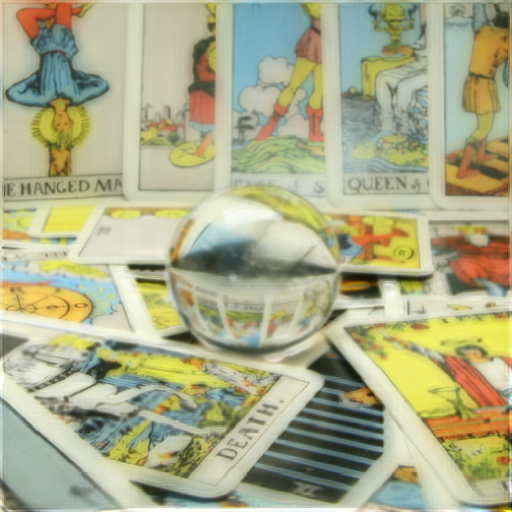
\includegraphics[width = 3.75cm]{../Figures/depth_compression/baseline_scaled_shifted/Reconstruction_of_view_(9,9).png}};
			\end{scope}	
		\end{tikzpicture}
	};
	\draw[blue] (box2.south east) rectangle (box2.north west);
			
	
	\end{tikzpicture}
\end{document}

		\caption{}
		\label{fig:reconstruction_baseline_scaled_shifted}
	\end{subfigure}
	\caption[Baseline scaling]
			{Depth compression by means of baseline scaling.
			 Shown is the reconstructed central angular view without proper baseline scaling (a) and with scaling (b).
			 The light field used is from the Stanford light field archive, \mbox{\url{http://lightfield.stanford.edu}}.}
	\label{fig:baseline_scaling}
\end{figure}
The reconstruction shows that cards in the front and back are blurred because the are virtually further away from the display, while the objects in the center are sharper.
\todo{Explain back-projection.}

\section{Attenuator Tiling and Blending}
\label{sec:tiling_and_blending}

High resolution light fields can take up a significant amount of space in memory. 
For example, a light field taken with a Full HD camera from $17 \times 17$ angles would take up $1920 \cdot 1080 \cdot 17^2 \cdot 3 \cdot 8 / (1024^3) = 13.3947$ Gigabyte of memory. 
In addition, the propagation matrix stores information about every pixel in the light field and thus, can take up Gigabytes of space depending on the resolution of the attenuation layers. 
The proposed approach divides the attenuation layers into tiles. 
Figure~\ref{fig:tiling_layout} shows how the tiles are laid out.
\begin{figure}[tb]
	\begin{subfigure}{0.5\textwidth}
		\centering
		\documentclass{standalone}
\usepackage{tikz}

\begin{document}
	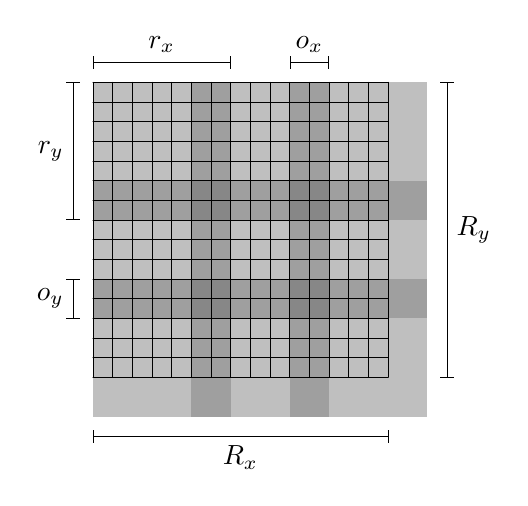
\begin{tikzpicture}[scale = 0.25, very thin]
	
		% Tiles
		\foreach \x in {0,...,2} {
			\foreach \y in {0,...,2}{
				\fill[gray, opacity = 0.5] (\x * 5, -\y * 5) rectangle ++(7, -7);
			}
		}
		
		% Grid
		\draw[step = 1 cm, cap = round] (0, 0) grid (15, -15);
		
		% Markers
		\draw[|-|] (0, -18) -- node[below]	{$R_x$} ++(15, 0);
		\draw[|-|] (18, 0) -- node[right]	{$R_y$} ++(0, -15);
		\draw[|-|] (0, 1) 	-- node[above]	{$r_x$} ++(7, 0);
		\draw[|-|] (-1, 0) 	-- node[left]	{$r_y$} ++(0, -7);
		\draw[|-|] (10, 1) 	-- node[above]	{$o_x$} ++(2, 0);
		\draw[|-|] (-1, -10) -- node[left]	{$o_y$} ++(0, -2);
	
	\end{tikzpicture}
\end{document}

		\caption{}
		\label{fig:tiling_layout}
	\end{subfigure}%
	\begin{subfigure}{0.5\textwidth}
		\centering
		\documentclass{standalone}
\usepackage{calc}
\usepackage{tikz}

\begin{document}
	\begin{tikzpicture}[scale = 0.25, very thin]
	
		% Tiles
%		\foreach \x in {0,...,2} {
%			\foreach \y in {0,...,2}{
%				\fill[gray, opacity = 0.5] (\x * 5, -\y * 5) rectangle ++(7, -7);
%			}
%		}

		% Summed up masks
		\node [anchor = north west, inner sep = 0] at (0, 0) {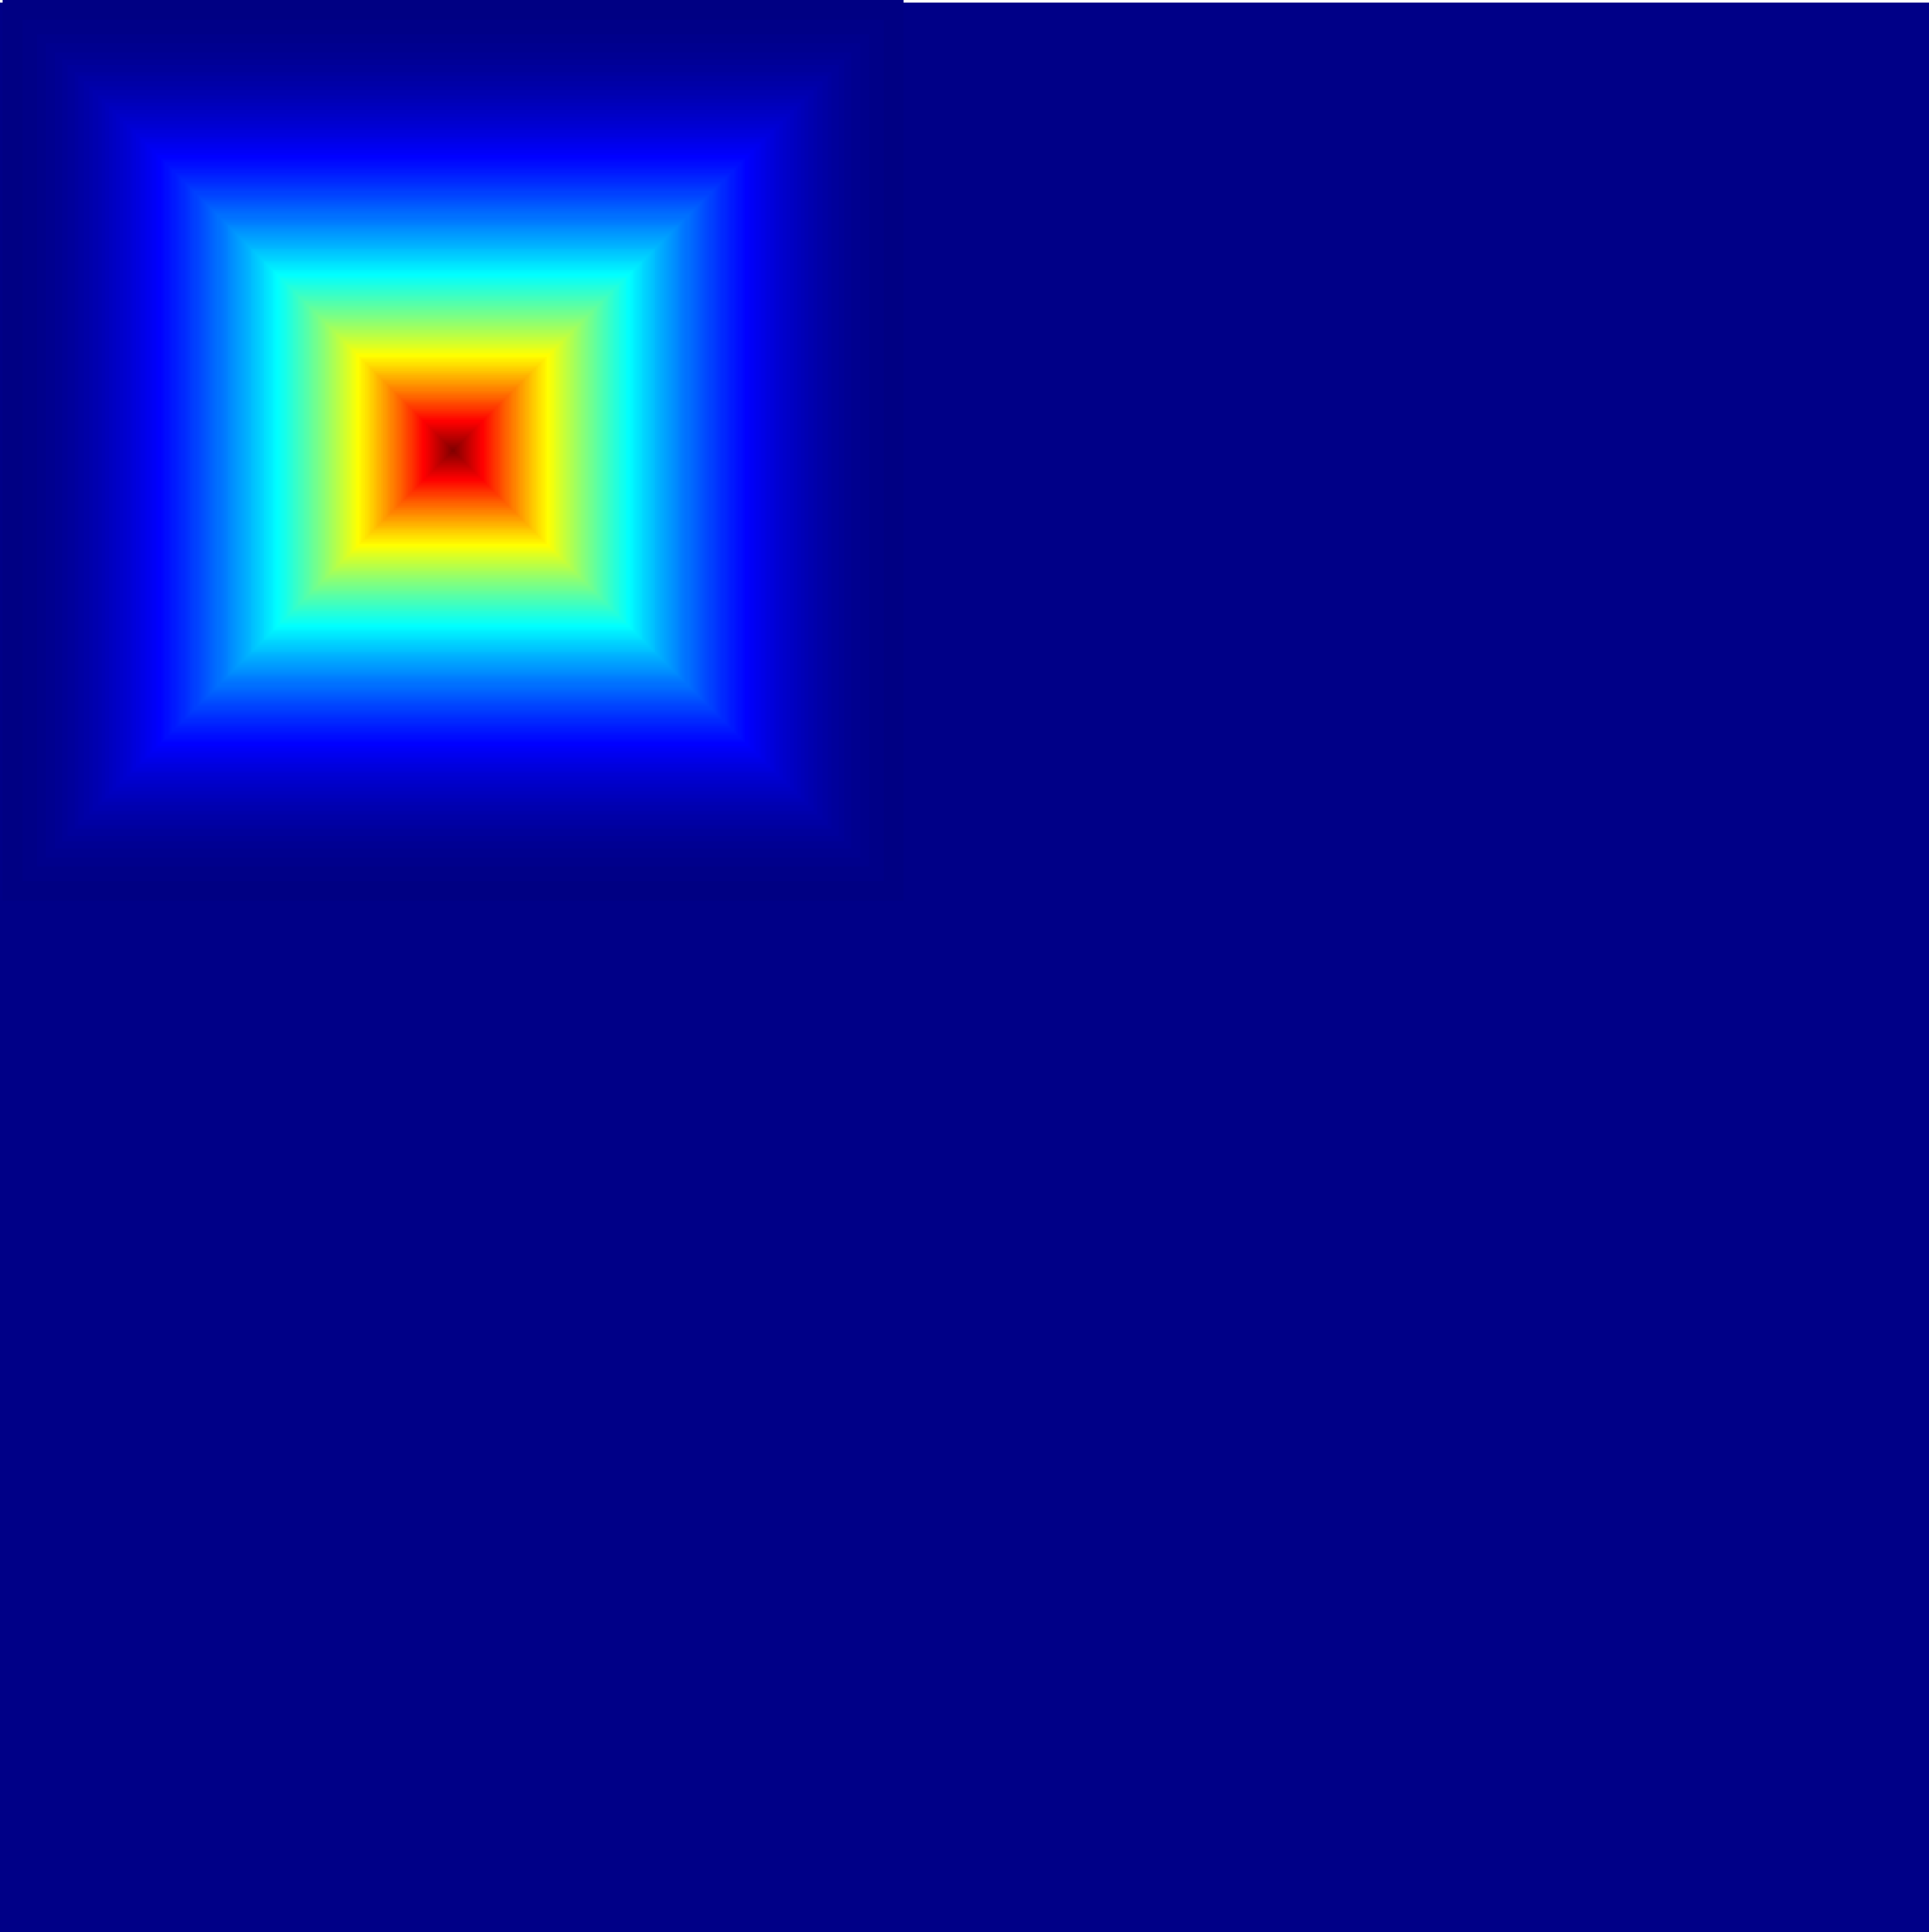
\includegraphics[width = 3.75cm]{./figures/tiling/mask1}};
		\node [anchor = east, scale=2] at (-0.5, -3.6) {$\ast$};
		% Grid
%		\draw[step = 1 cm, cap = round] (0, 0) grid (15, -15);
		
		% Invisible markers for accurate placement in figure 
		\begin{scope}[opacity = 0]
			\draw[|-|] (0, -18) -- node[below]	{$R_x$} ++(15, 0);
%			\draw[|-|] (18, 0) -- node[right]	{$R_y$} ++(0, -15);
			\draw[|-|] (0, 1) 	-- node[above]	{$r_x$} ++(7, 0);
%			\draw[|-|] (-1, 0) 	-- node[left]	{$r_y$} ++(0, -7);
			\draw[|-|] (10, 1) 	-- node[above]	{$o_x$} ++(2, 0);
%			\draw[|-|] (-1, -10) -- node[left]	{$o_y$} ++(0, -2);
		\end{scope}
		
	\end{tikzpicture}
\end{document}
		\caption{}
		\label{fig:sum_of_quadratic_blending_masks}
	\end{subfigure}%
	\caption[Tiling layout]
			{(a) Layout of the tiles that cover the attenuation layers.
				 The pixel grid of size $R_x \times R_y$ is covered by tiles of $r_x \times r_y$ pixels with an overlap of $o_x$ in horizontal and $o_y$ in vertical direction.
			 (b) The sum of the per-tile quadratic blending masks used for the normalization.}
\end{figure} 
The inputs for the tiling algorithm are the resolution of the tiles $r = (r_x, r_y)$ and the overlap in horizontal and vertical direction, $o = (o_x, o_y)$. 
The tiles are then laid out in a grid beginning in the top left corner of the layer. 
The number of tiles needed to cover the plane can be calculated by 
\begin{equation}
	N_x = \left \lceil \dfrac{R_x - o_x}{r_x - o_x} \right \rceil
	\qquad 
	\text{and} 
	\qquad
	N_y = \left \lceil \dfrac{R_y - o_y}{r_y - o_y} \right \rceil.
\end{equation}
The combination of the same tile from each layer forms a new attenuator of smaller size and lower resolution. 
The optimization is then performed for every tile separately, resulting in a smaller propagation matrix per tile. 
In the end, the optimized tiles are put together to form the complete attenuation layers. 

In general, the borders of the attenuator contain less ray-propagation information and thus provide a higher degree of freedom for the optimization. 
This introduces artifacts that are clearly visible in the reassembled layers as shown in figure~\ref{fig:comparison_tile_overlap_vs_no_overlap}.
\begin{figure}[tb]
	\centering
	\begin{subfigure}{0.23\textwidth}
		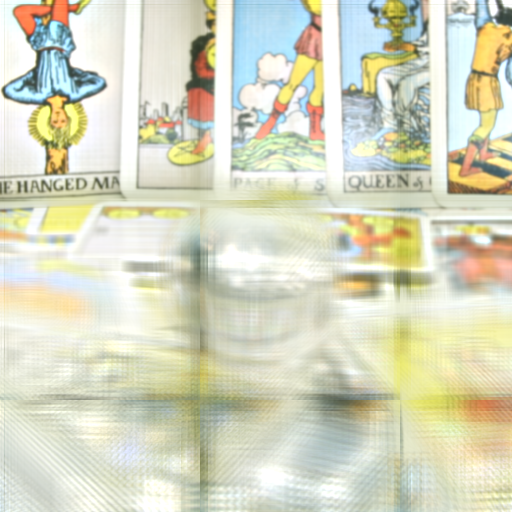
\includegraphics[width = \textwidth]{../Figures/tiling/tarot_tiles3x3x200x200_no_overlap_3_layers/1.png}
		
		\vspace{0.15cm}
		
		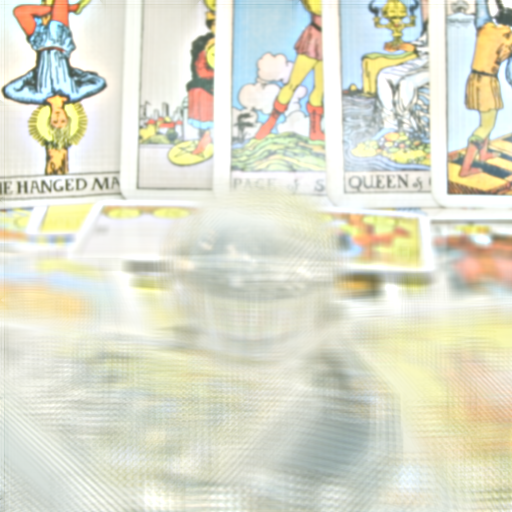
\includegraphics[width = \textwidth]{../Figures/tiling/tarot_tiles5x5x200x200_overlap0.5_3_layers/1.png}
		\caption{Layer 1}
	\end{subfigure}\hspace{0.15cm}%
	\begin{subfigure}{0.23\textwidth}
		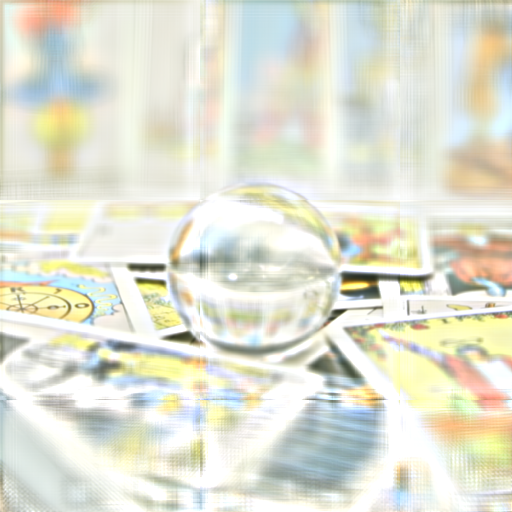
\includegraphics[width = \textwidth]{../Figures/tiling/tarot_tiles3x3x200x200_no_overlap_3_layers/2.png}
		
		\vspace{0.15cm}
		
		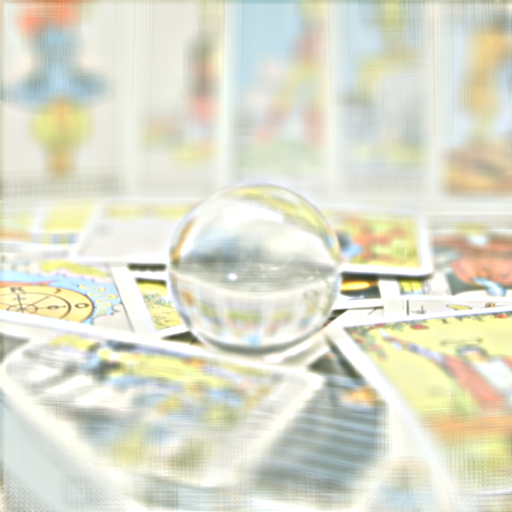
\includegraphics[width = \textwidth]{../Figures/tiling/tarot_tiles5x5x200x200_overlap0.5_3_layers/2.png}
		\caption{Layer 2}
	\end{subfigure}\hspace{0.15cm}%
	\begin{subfigure}{0.23\textwidth}
		
\includegraphics[width = \textwidth]{../Figures/tiling/tarot_tiles3x3x200x200_no_overlap_3_layers/3.png}
		
		\vspace{0.15cm}
		
		
\includegraphics[width = \textwidth]{../Figures/tiling/tarot_tiles5x5x200x200_overlap0.5_3_layers/3.png}
		\caption{Layer 3}
	\end{subfigure}\hspace{0.15cm}%
	\begin{subfigure}{0.23\textwidth}
		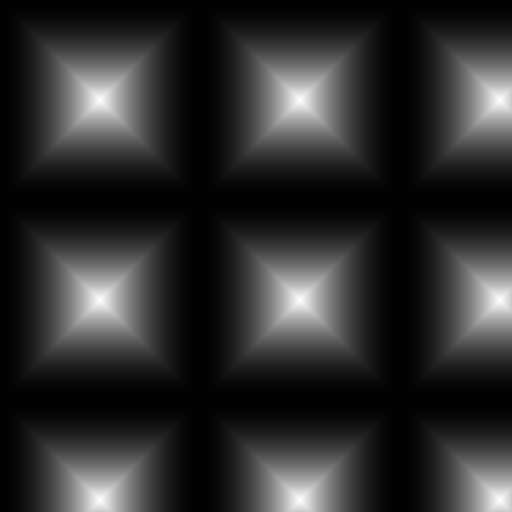
\includegraphics[width = \textwidth]{../Figures/tiling/tarot_tiles3x3x200x200_no_overlap_3_layers/blendingMaskSum.png}
		
		\vspace{0.15cm}
		
		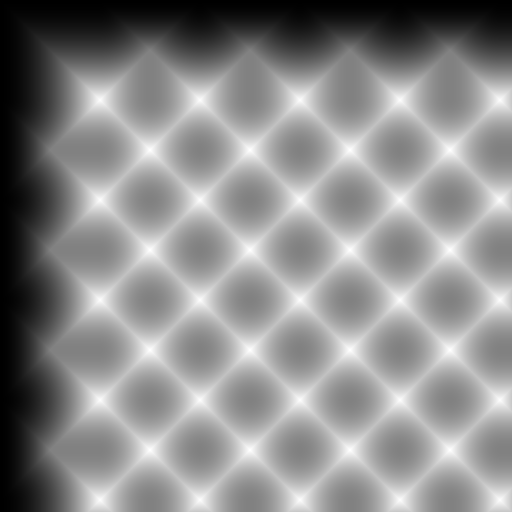
\includegraphics[width = \textwidth]{../Figures/tiling/tarot_tiles5x5x200x200_overlap0.5_3_layers/blendingMaskSum.png}
		\caption{Blending masks}
	\end{subfigure}%
	\caption[Impact of tile overlap on attenuation layers]
			{Impact of tile overlap on attenuation layers.
			 Top: Tiles have no overlap and grid artifacts are visible.
			 Bottom: With a 50\% overlap, the artifacts are no longer noticeable, but more tiles are needed.}
	\label{fig:comparison_tile_overlap_vs_no_overlap}
\end{figure} 
To solve this issue, the tiles have to overlap. 
In this case, when reassembling the layers from the tiles, the overlaps need to be blended with a mask:
After the optimization, each tile gets multiplied with a quadratic blending mask.
The finished layers are then obtained by summing the tiles and dividing by the sum of the blending masks shown in figure~\ref{fig:sum_of_quadratic_blending_masks}.

\todo{choice of quadratic masks?}

\section{Performance of SART}
\label{sec:performance_of_SART}

\todo{fix gridlines in figure!}

\begin{figure}[tb]
	\begin{subfigure}{0.5\textwidth}
		\centering
		\documentclass{standalone}
\usepackage{pgfplots}

\begin{document}
	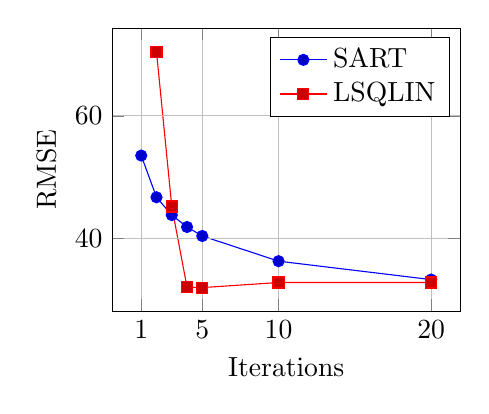
\begin{tikzpicture}
		
		\begin{axis}[	legend pos = north east, 
						legend cell align = left,
						xtick = {1, 5, 10, 20},
						ylabel = {RMSE},
						xlabel = {Iterations},
						ylabel near ticks,
						grid = major,
						axis on top = true,
						width = 6 cm]
		
			\addplot coordinates {
				(1, 53.517116)
				(2, 46.6983)
				(3, 43.7923)
				(4, 41.8413)
				(5, 40.3709)
				(10, 36.2524)
				(20, 33.2420)
			};
			\addlegendentry{SART};
			
			\addplot coordinates {
				(2, 70.477447)
				(3, 45.188843)
				(4, 32.001308)
				(5, 31.934515)
				(10, 32.764468)
				(20, 32.766828)
			};
			\addlegendentry{LSQLIN};
			
			 
		\end{axis}
		
	\end{tikzpicture}
\end{document}
		\caption{}
		\label{fig:sart_lsqlin_iterations_vs_rmse}
	\end{subfigure}%
	\begin{subfigure}{0.5\textwidth}
		\centering
		\documentclass{standalone}
\usepackage{pgfplots}

\begin{document}
	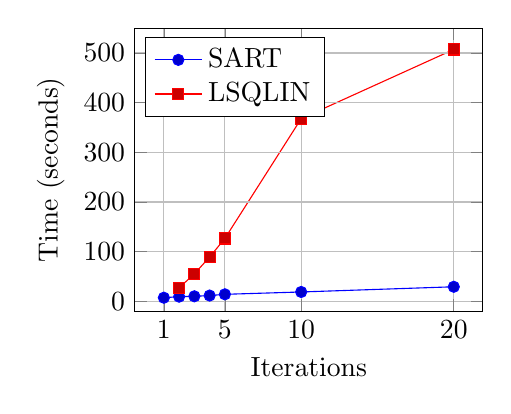
\begin{tikzpicture}
		
		\begin{axis}[	legend pos = north west, 
						legend cell align = left,
						ymin = -20,
						ymax = 550,
						xtick = {1, 5, 10, 20},
						ytick = {0, 100, 200, 300, 400, 500},
						ylabel = {Time (seconds)},
						xlabel = {Iterations},
						ylabel near ticks,
						grid,
						axis on top = true,
						width = 6 cm]
		
			\addplot coordinates {
				(1, 7.0933)
				(2, 9.2096)
				(3, 9.9564)
				(4, 11.4550)
				(5, 13.9412)
				(10, 18.6697)
				(20, 29.1313)
			};
			\addlegendentry{SART};
			
			\addplot coordinates {
				(2, 26.9930)
				(3, 55.2522)
				(4, 89.0784)
				(5, 126.5243)
				(10, 367.7888)
				(20, 507.2163)
			};
			\addlegendentry{LSQLIN};
			
			 
		\end{axis}
		
	\end{tikzpicture}
\end{document}
		\caption{}
		\label{fig:sart_lsqlin_iterations_vs_time}
	\end{subfigure}%
	\caption[Performance assessment of the optimization]
			{Performance assessment of the optimization.
			 The two iterative methods \mbox{SART} and \mbox{MATLAB's} linear least squares solver \emph{lsqlin} are compared in terms of \mbox{RMSE} (a) and runtime (b).
			 The input light field is the same as in figure~\ref{fig:baseline_scaling} and five attenuation layers were used.}
	\label{fig:sart_vs_lsqlin}
\end{figure}

\begin{figure}[tb]
	\begin{subfigure}{\textwidth}
		\centering
		\documentclass{standalone}
\usepackage{pgfplots}

\begin{document}
	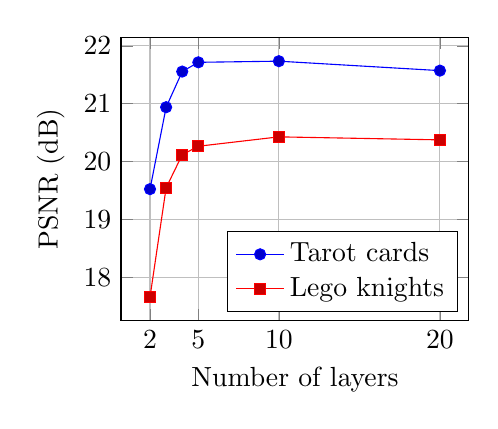
\begin{tikzpicture}
		
		\begin{axis}[	legend pos = south east, 
						legend cell align = left,
						xtick = {2, 5, 10, 20},
						ytick = {18, 19, 20, 21, 22},
						ylabel = {PSNR (dB)},
						xlabel = {Number of layers},
						ylabel near ticks,
						grid,
						axis on top = false,
						width = 6 cm]
						
		%% NOTE: I added the 4.7712 = 10 * log_10(3) because I forgot to normalize the MSE by the number of color channels 
		
			\addplot coordinates {
				(2, 14.7555 + 4.7712)
				(3, 16.1691 + 4.7712)
				(4, 16.7842 + 4.7712)
				(5, 16.9441 + 4.7712)
				(10, 16.9636 + 4.7712)
				(20, 16.8005 + 4.7712)
			};
			\addlegendentry{Tarot cards};
			
			\addplot coordinates {
				(2, 12.8945 + 4.7712)
				(3, 14.7783 + 4.7712)
				(4, 15.3490 + 4.7712)
				(5, 15.4956 + 4.7712)
				(10, 15.6576 + 4.7712)
				(20, 15.6058 + 4.7712)
			};
			\addlegendentry{Lego knights};
			
			 
		\end{axis}
		
	\end{tikzpicture}
\end{document}
		\caption{SART}
		\label{fig:sart_layers_vs_psnr}
	\end{subfigure}%
	\caption[Impact of layer count on \mbox{PSNR}]
			{Impact of layer count on the \mbox{PSNR}.
			 Performance comparison of the attenuation display for two different scenes from the Stanford light field archive.
			 The \mbox{PSNR} is evaluated against the number of layers.}
\end{figure}

\section{Benefits and Limitations}
\label{sec:benefits_limitations}

\todo{Optimization only for positive transmittance}
